% @Author: Athul Vijayan
% @Date:   2014-05-09 13:56:20
% @Last Modified by:   athul
% @Last Modified time: 2015-09-13 13:16:33

\documentclass[11pt]{article}
\usepackage[utf8]{inputenc}
\usepackage[a4paper, margin=1in]{geometry}
\usepackage{amsmath}
\usepackage[table]{xcolor}
\usepackage{amssymb}
\usepackage{graphicx}
\usepackage[toc,page]{appendix}
\usepackage{color}
\usepackage{subcaption}
\usepackage{placeins}
\usepackage{rotating}
\usepackage{wrapfig}
\usepackage{bm}
\usepackage[normalem]{ulem}
\usepackage[table]{xcolor}
\newcommand{\HRule}{\rule{\linewidth}{0.2mm}} % Defines a new command for the horizontal lines, change thickness here
\usepackage{hyperref}
\hypersetup{
    colorlinks,
    citecolor=black,
    filecolor=black,
    linkcolor=black,
    urlcolor=cyan
}
\usepackage{array}
\renewcommand{\P}{\mathbb{P}}
\newcolumntype{L}[1]{>{\raggedright\let\newline\\\arraybackslash\hspace{0pt}}m{#1}}
\newcolumntype{C}[1]{>{\centering\let\newline\\\arraybackslash\hspace{0pt}}m{#1}}
\newcolumntype{R}[1]{>{\raggedleft\let\newline\\\arraybackslash\hspace{0pt}}m{#1}}
\newcommand{\rulesep}{\unskip\ \vrule\ }

%----------------------------------------------------------------------------------------
%   TITLE PAGE
%----------------------------------------------------------------------------------------

\newcommand*{\titleGM}{\begingroup % Create the command for including the title page in the document
\hbox{ % Horizontal box
\hspace*{0.20.8\textwidth} % Whitespace to the left of the title page
\rule{1pt}{\textheight} % Vertical line
\hspace*{0.050.8\textwidth} % Whitespace between the vertical line and title page text
\parbox[b]{0.750.8\textwidth}{ % Paragraph box which restricts text to less than the width of the page

{\noindent\Huge\bfseries  Neural data analysis}\\[2\baselineskip] % Title
{\large \textit{Notes}}\\[4\baselineskip] % Tagline or further description
{\Large \textsc{Athul Vijayan \hspace{5pt} ed11b004}} % Author name

\vspace{0.5\textheight} % Whitespace between the title block and the publisher
}}
\endgroup}


\begin{document}
% \titleGM % This command includes the title page
\tableofcontents

% =========================== content =========================
\newpage
{\Large \textbf{Proof of resume points - ED11B004}
\FloatBarrier
\section{10th Marks}
\begin{figure}[h]
\centering
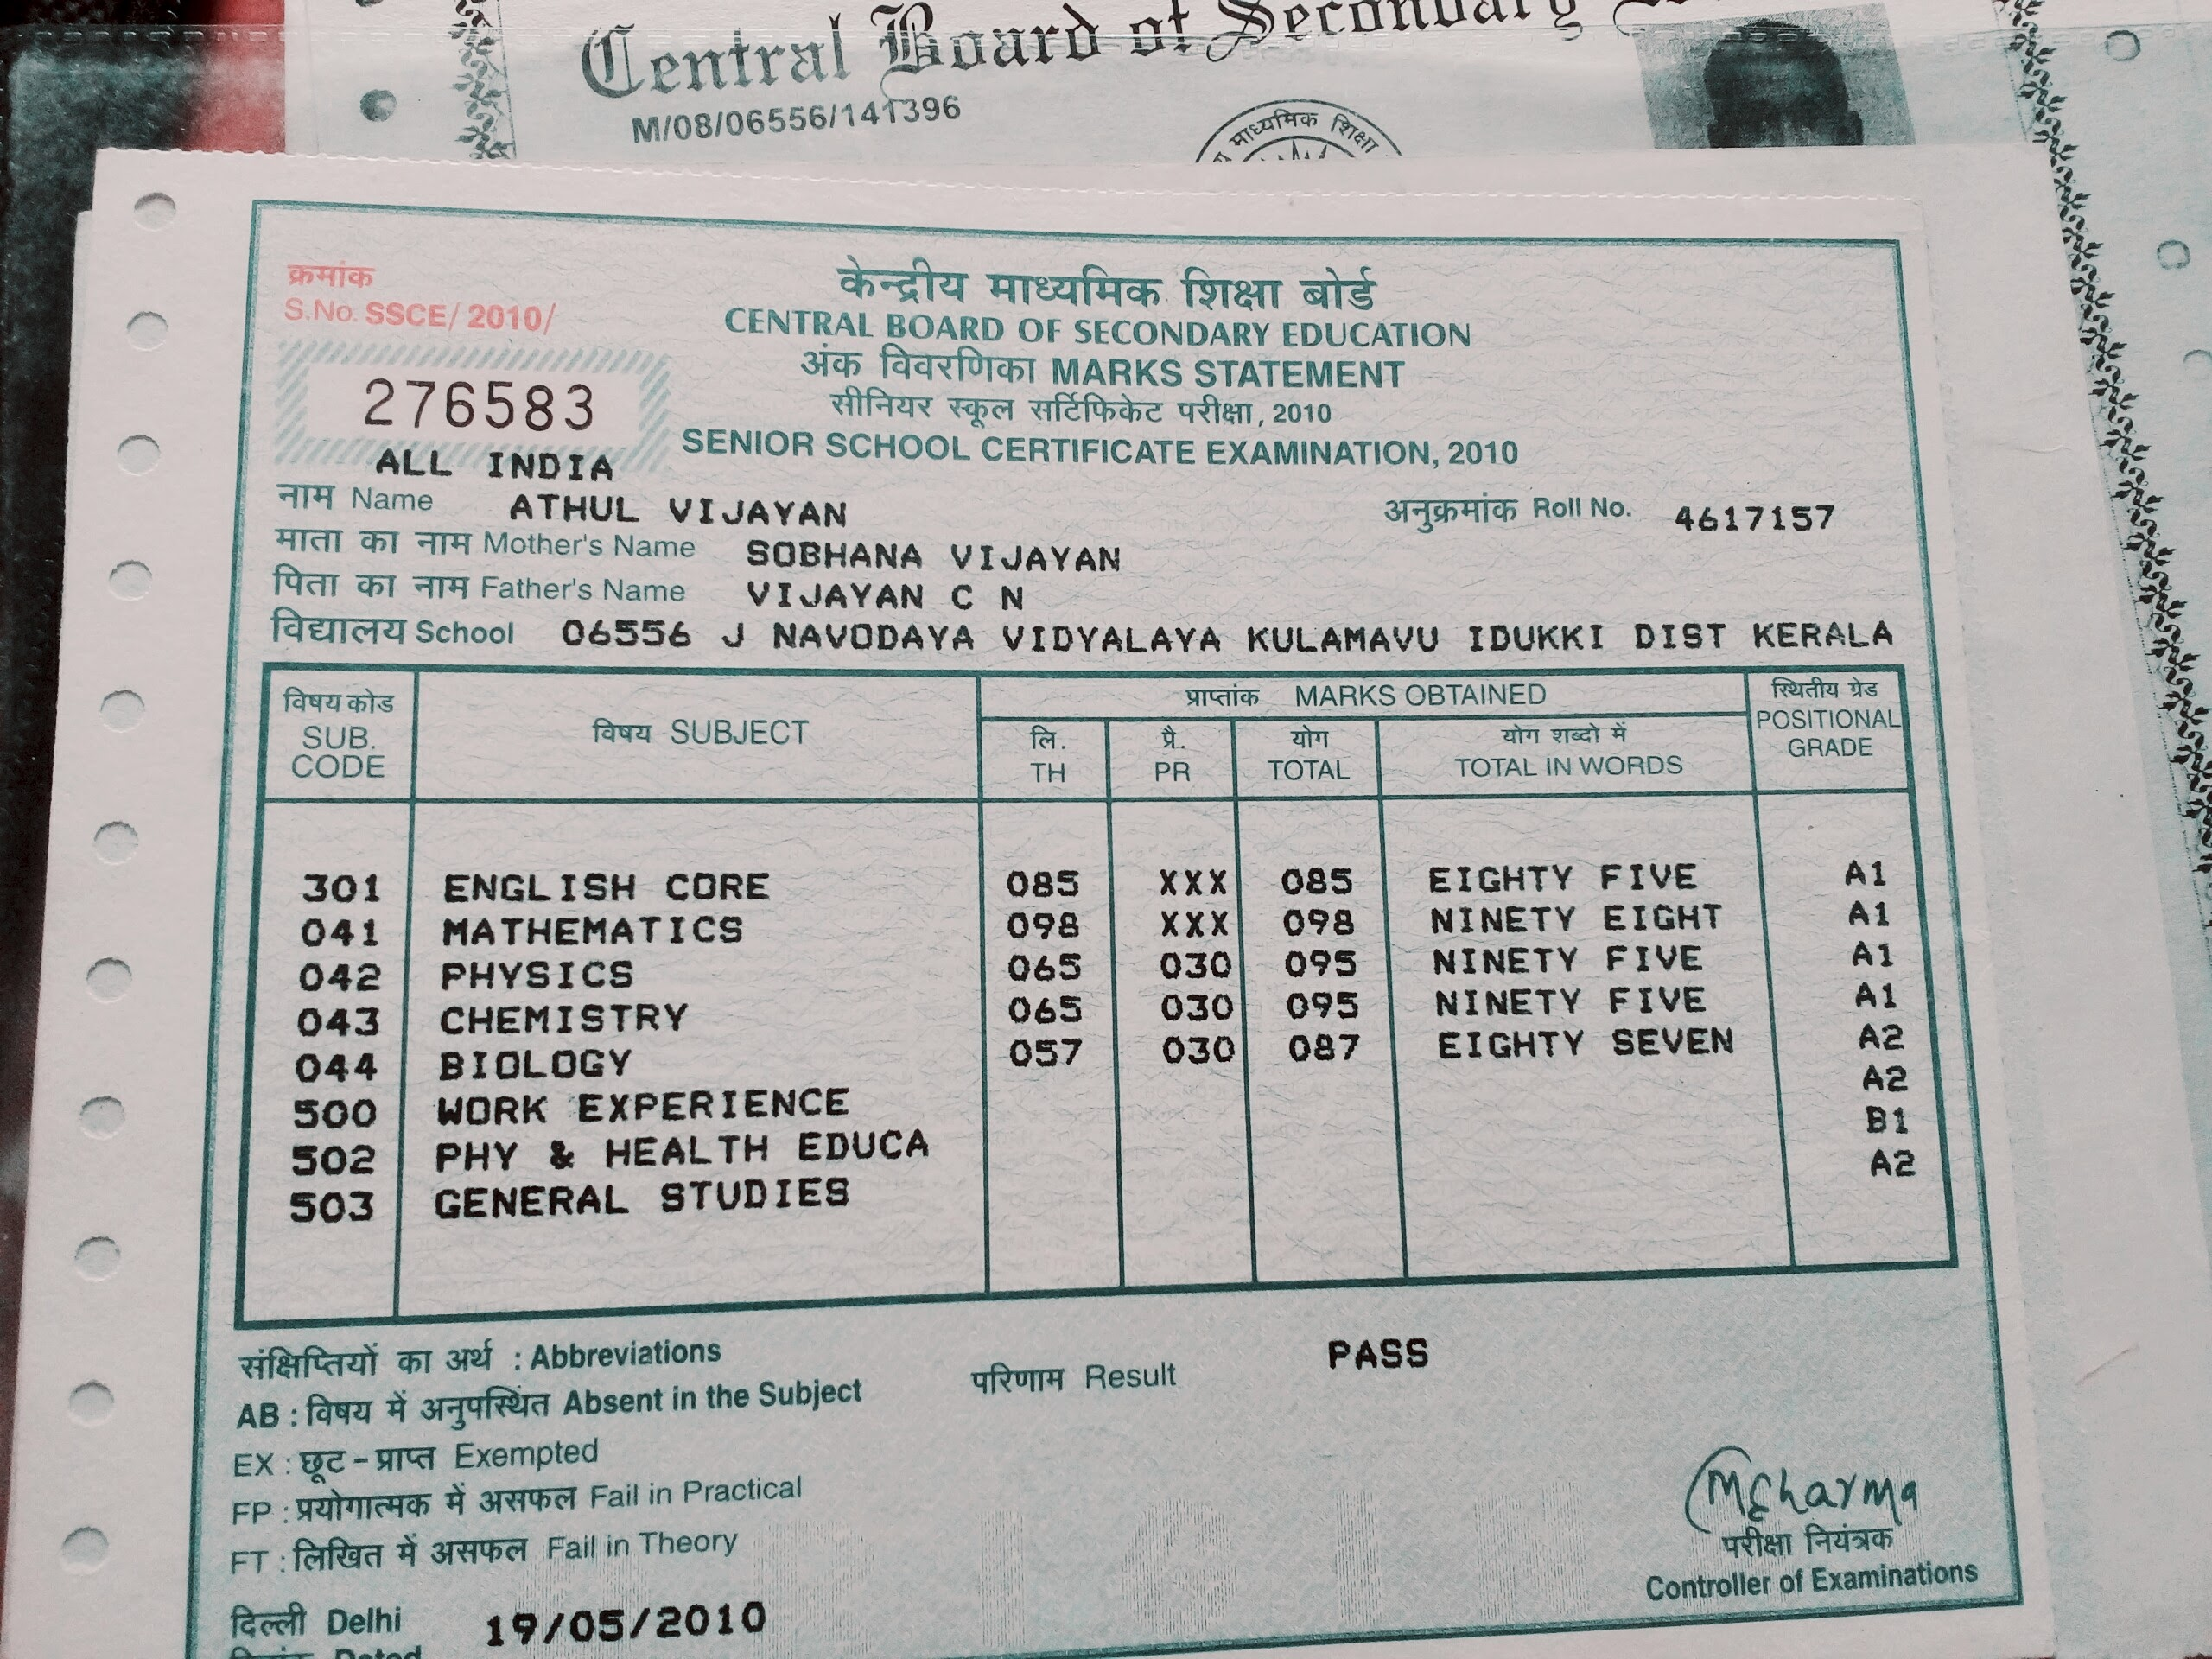
\includegraphics[width=0.8\textwidth]{10m.jpg}
\caption{10th mark list}
\label{gauss}
\end{figure}
\FloatBarrier
\section{12th Marks}
\begin{figure}[h]
\centering
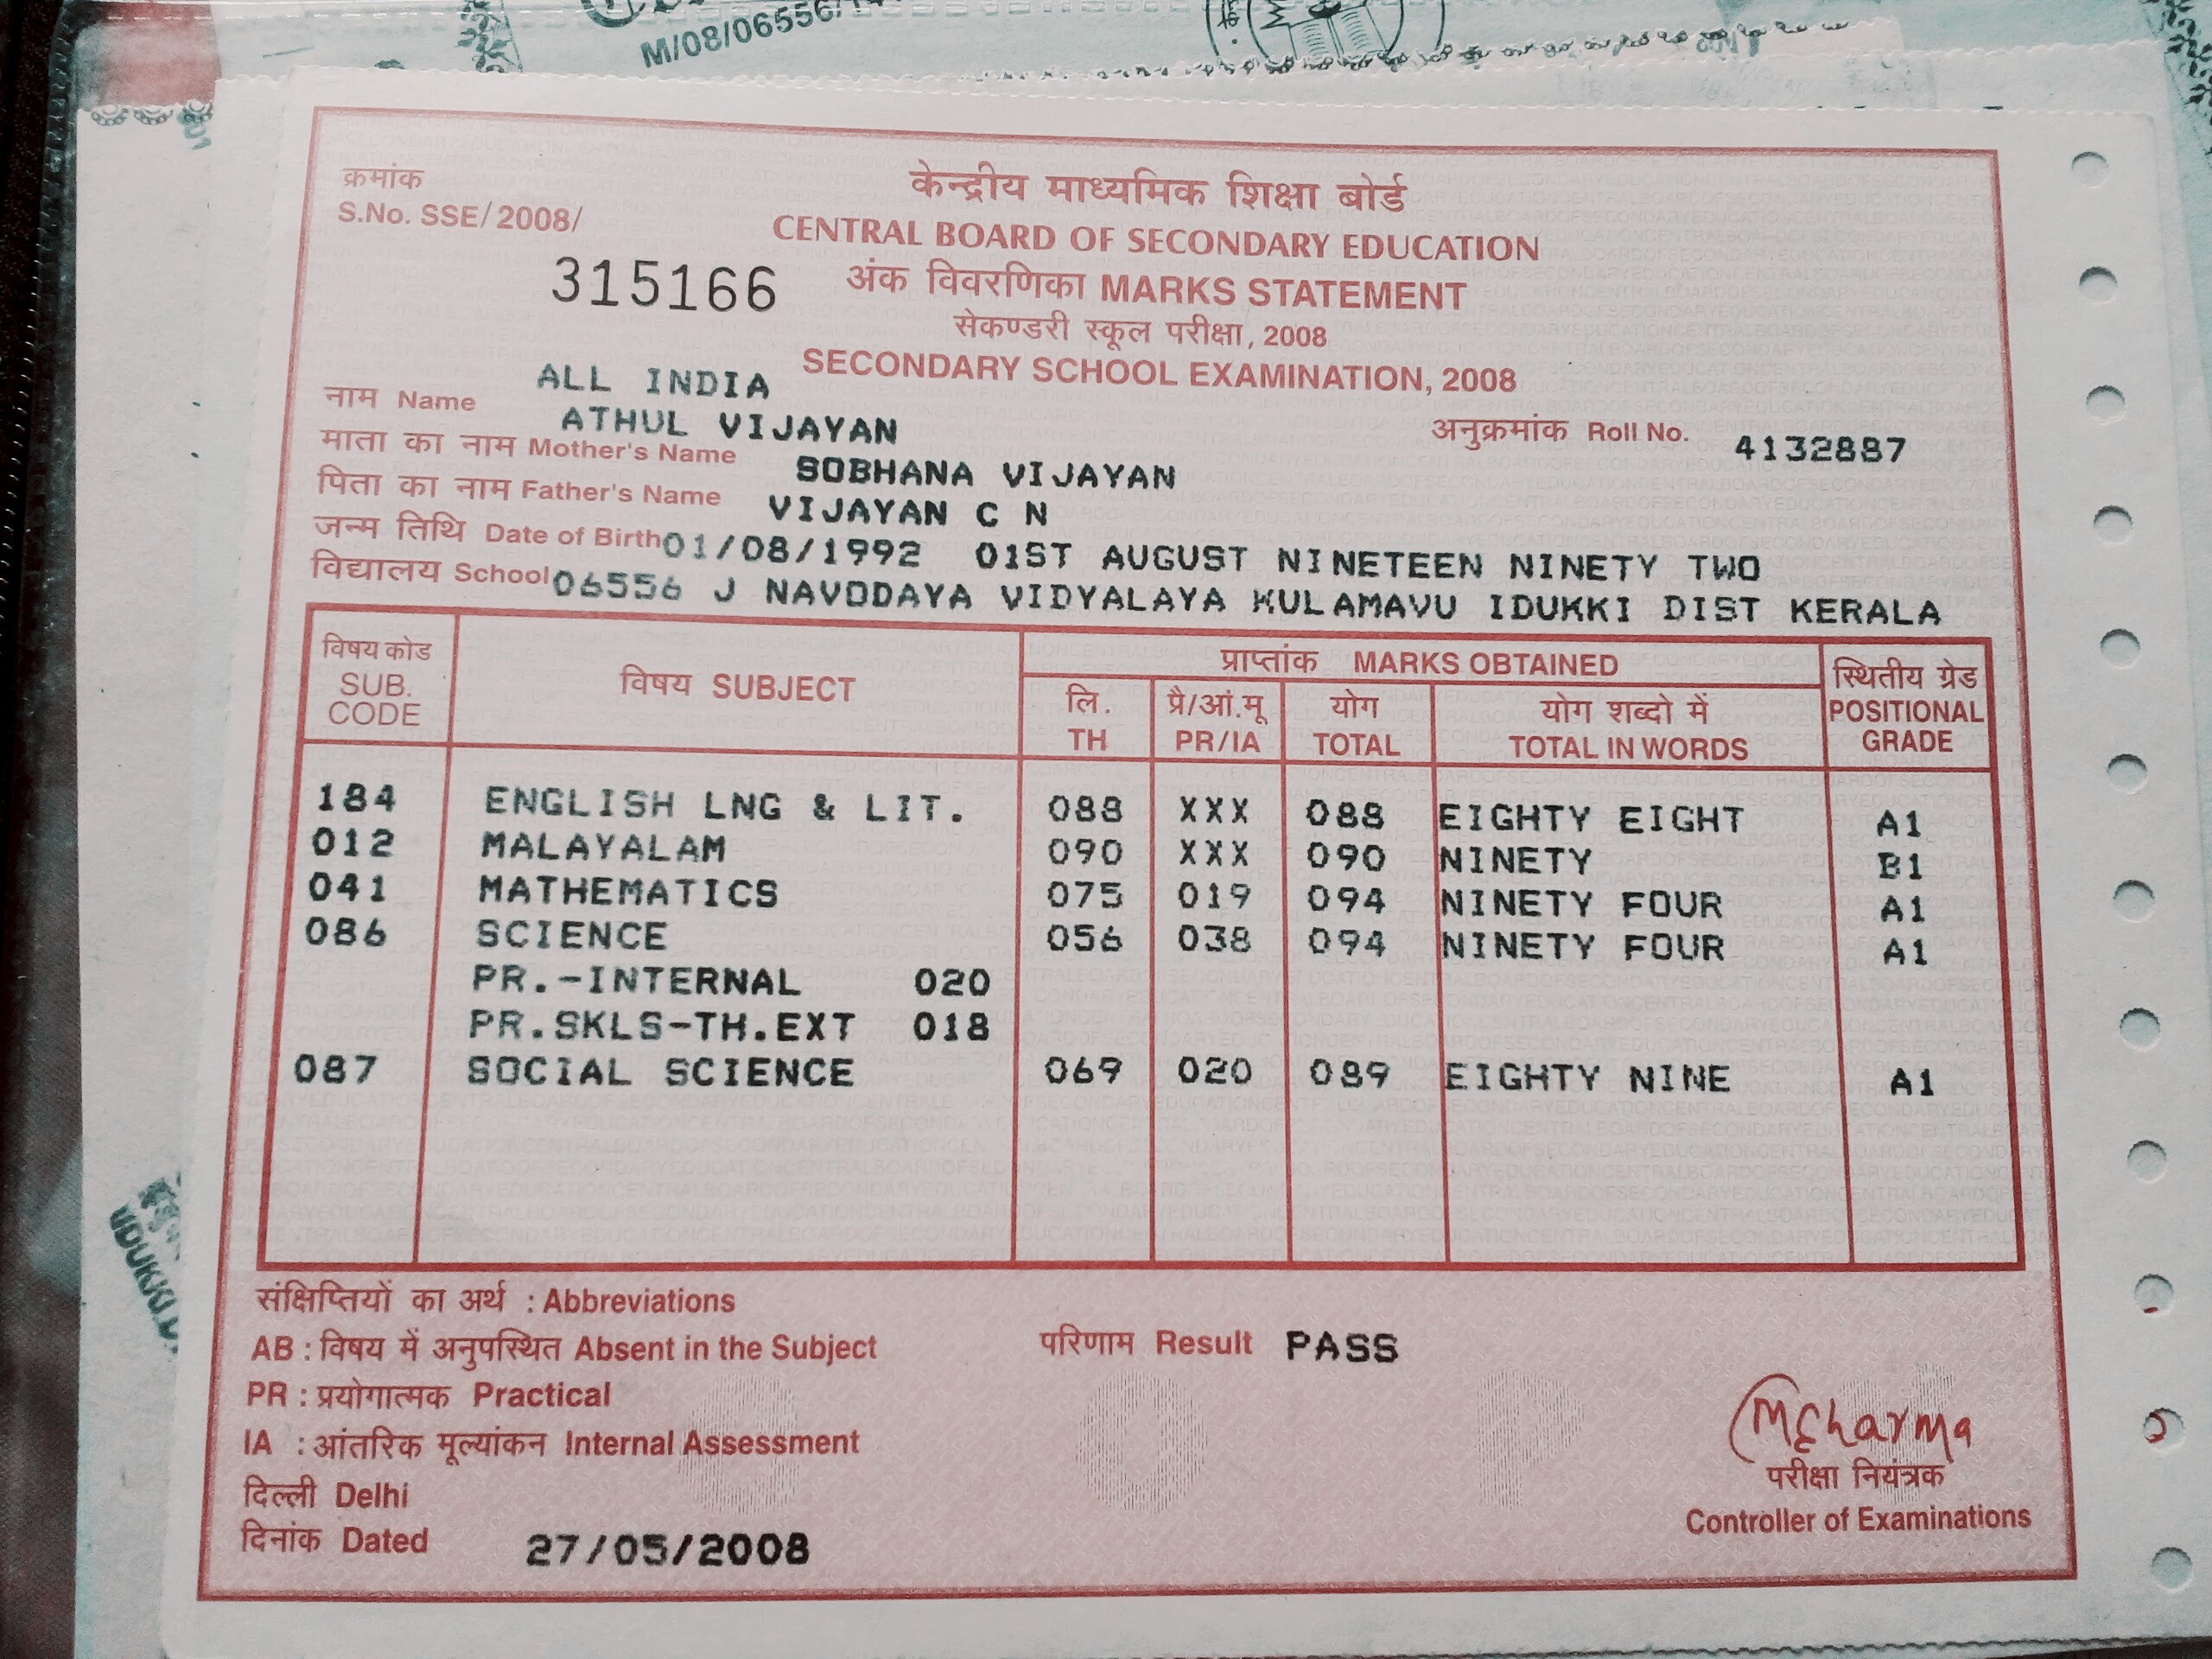
\includegraphics[width=0.8\textwidth]{12m.jpg}
\caption{12th mark list}
\label{gauss}
\end{figure}
\FloatBarrier
\section{JEE rank}
\begin{figure}[h]
\centering
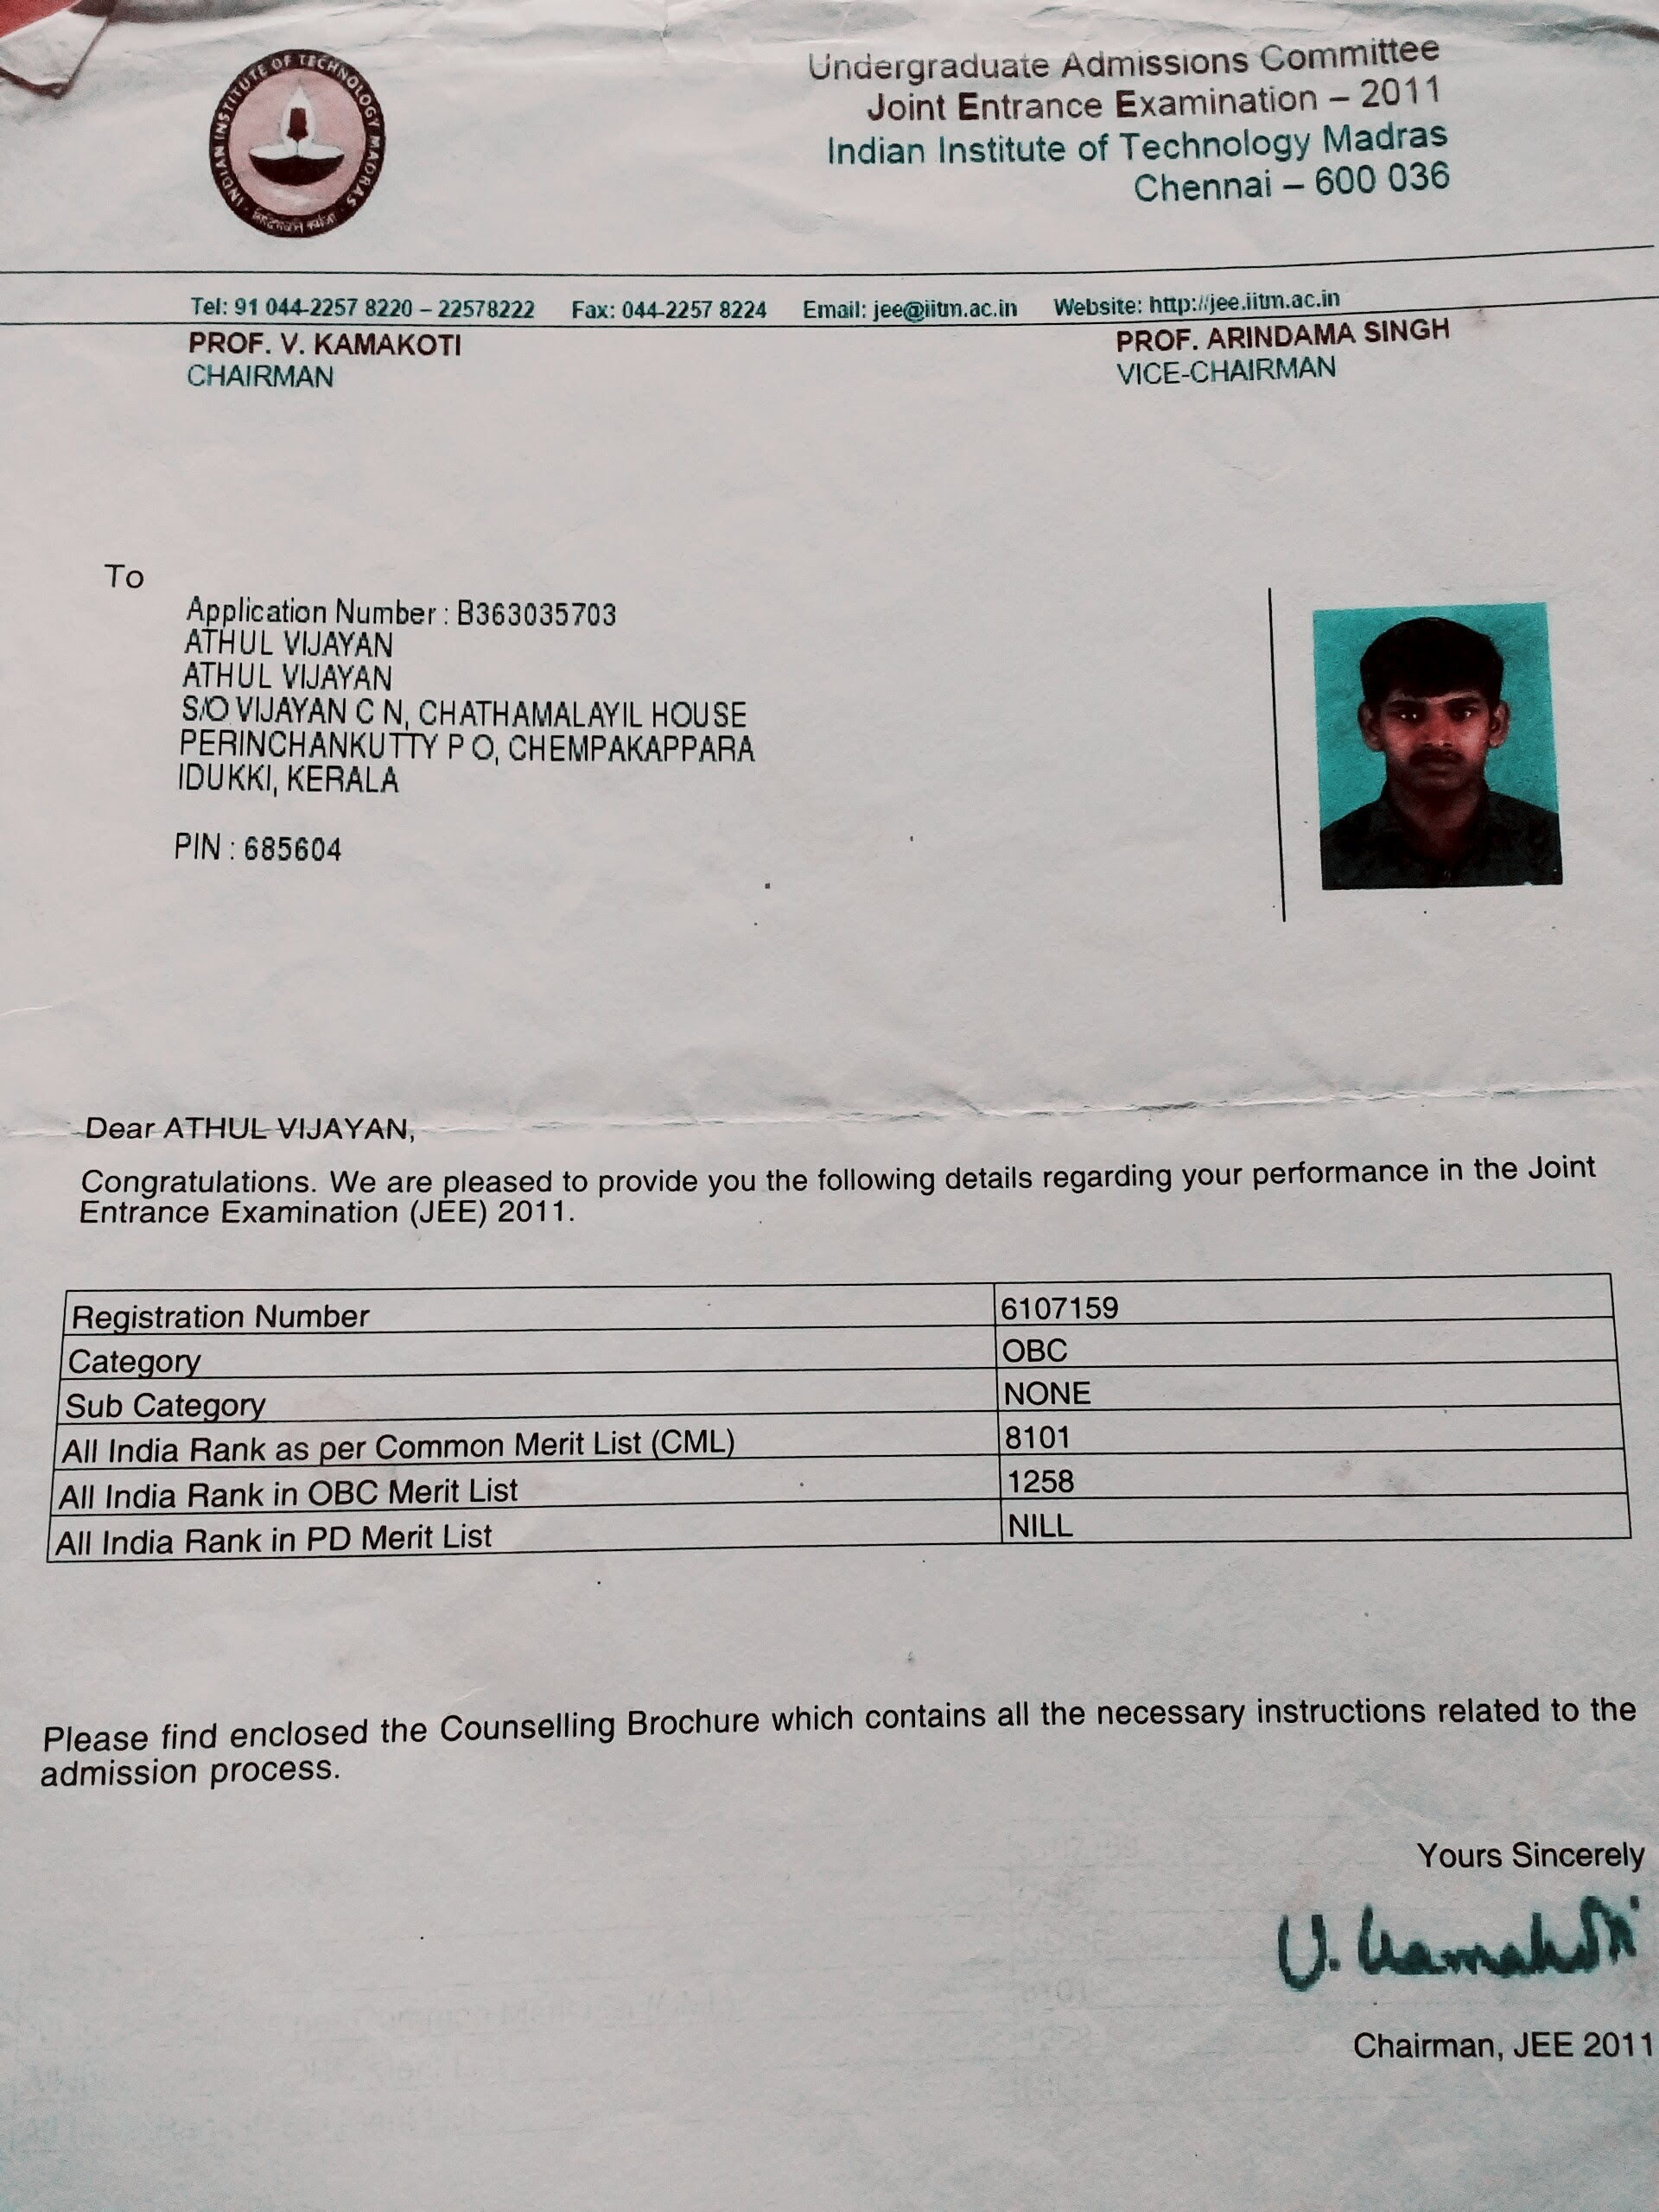
\includegraphics[width=0.8\textwidth]{jee.jpg}
\caption{JEE rank}
\label{gauss}
\end{figure}
\FloatBarrier

\section{NI Intern}
\begin{figure}[h]
\centering
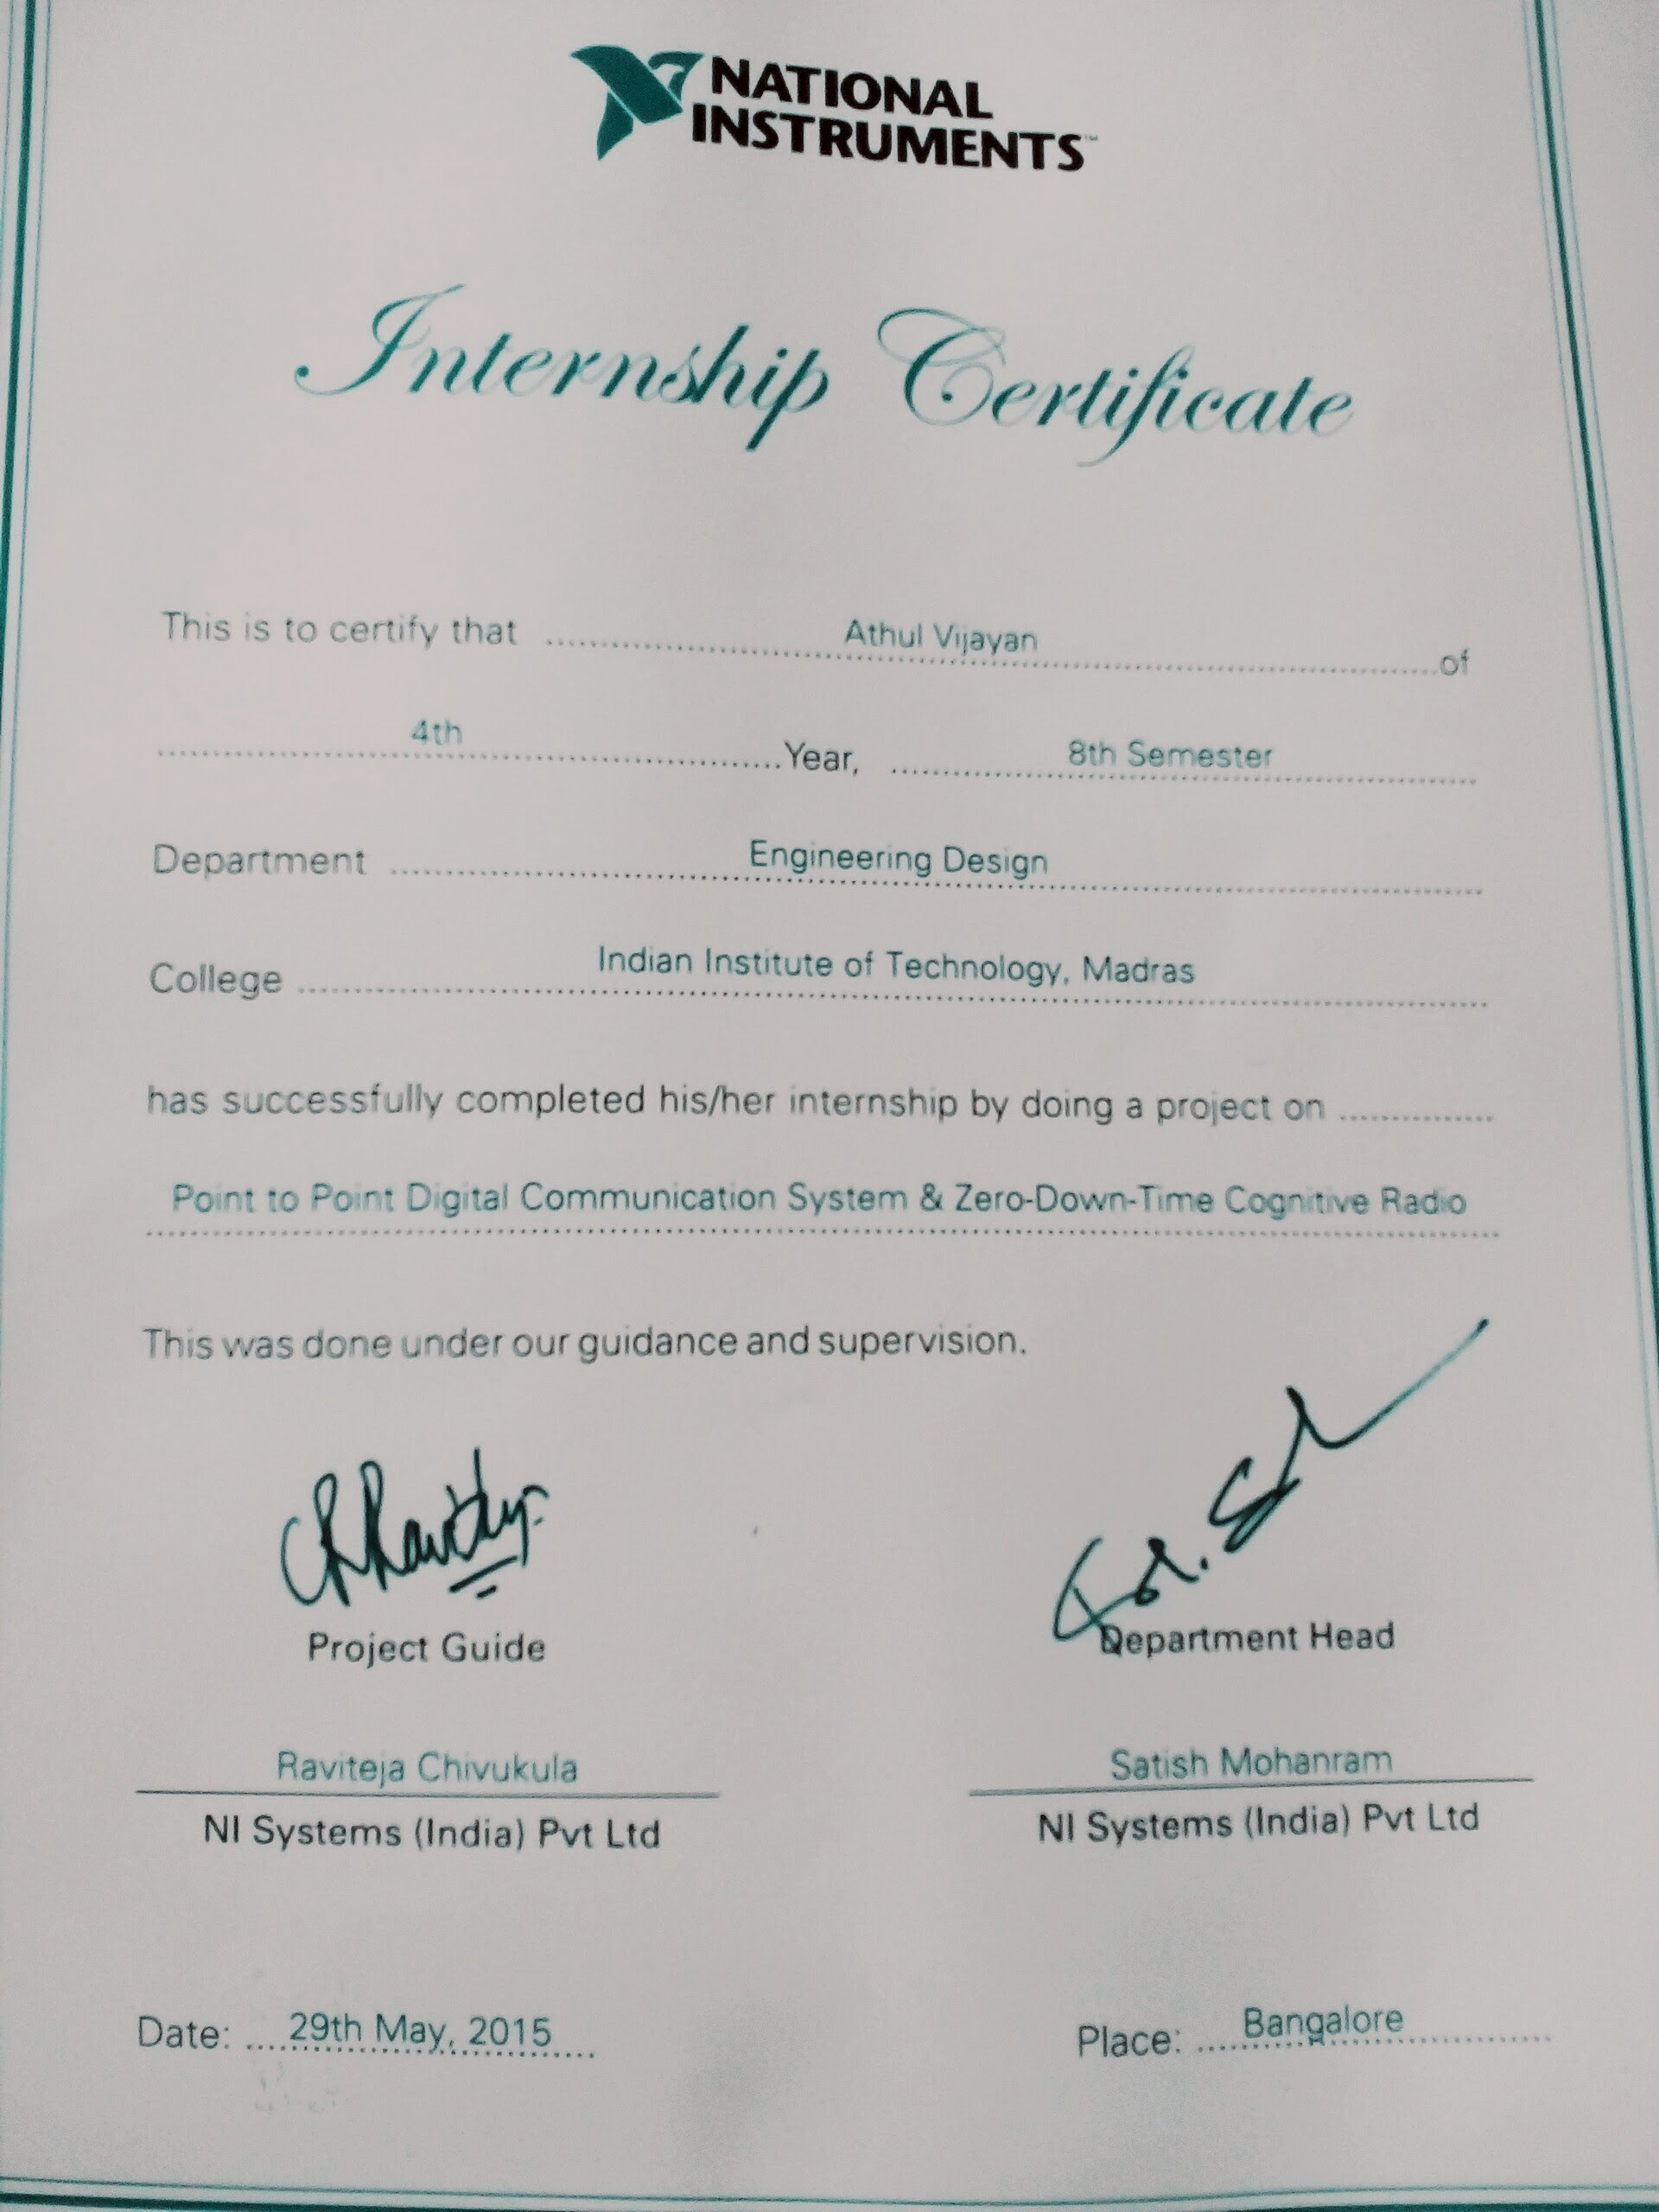
\includegraphics[width=0.8\textwidth]{ni.jpg}
\caption{NI Intern}
\label{gauss}
\end{figure}
\FloatBarrier

\section{ICSR project review notice}
\begin{figure}[h]
\centering
\begin{subfigure}{.48\textwidth}
    \centering
    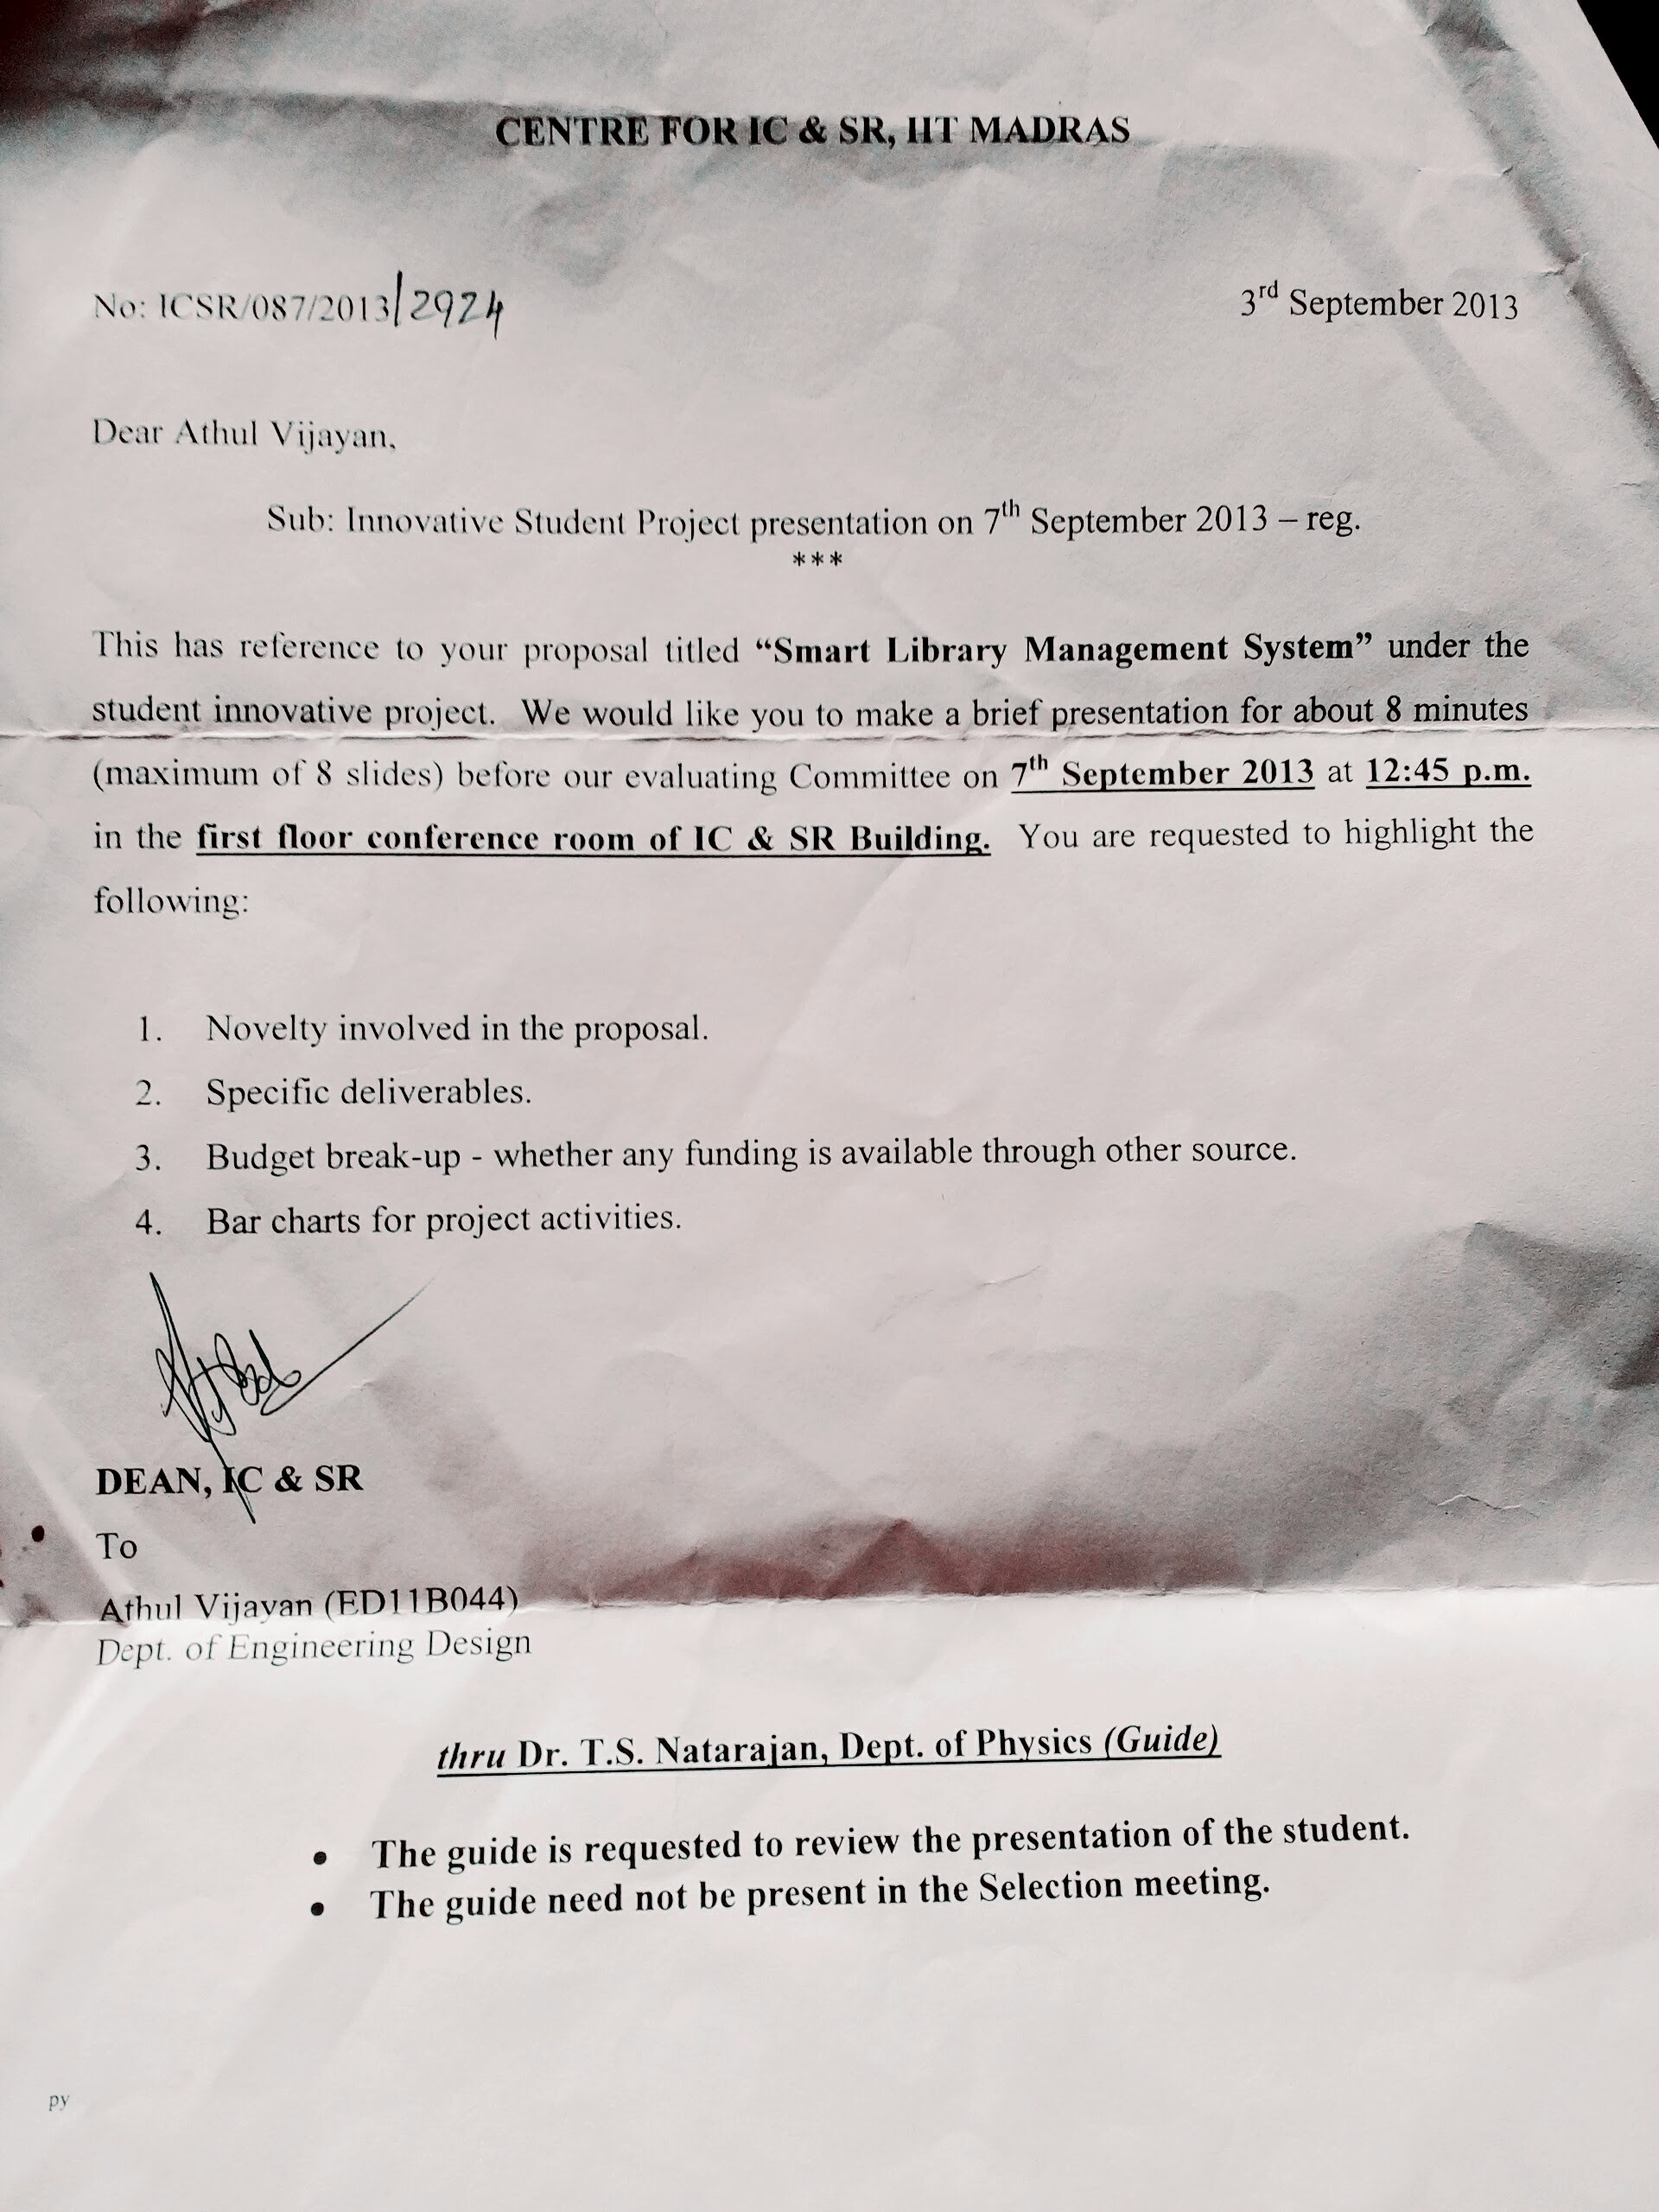
\includegraphics[width=\linewidth]{icsr.jpg}
    \caption{proposal intimdation}
\end{subfigure}
\rulesep
\begin{subfigure}{.48\textwidth}
    \centering
    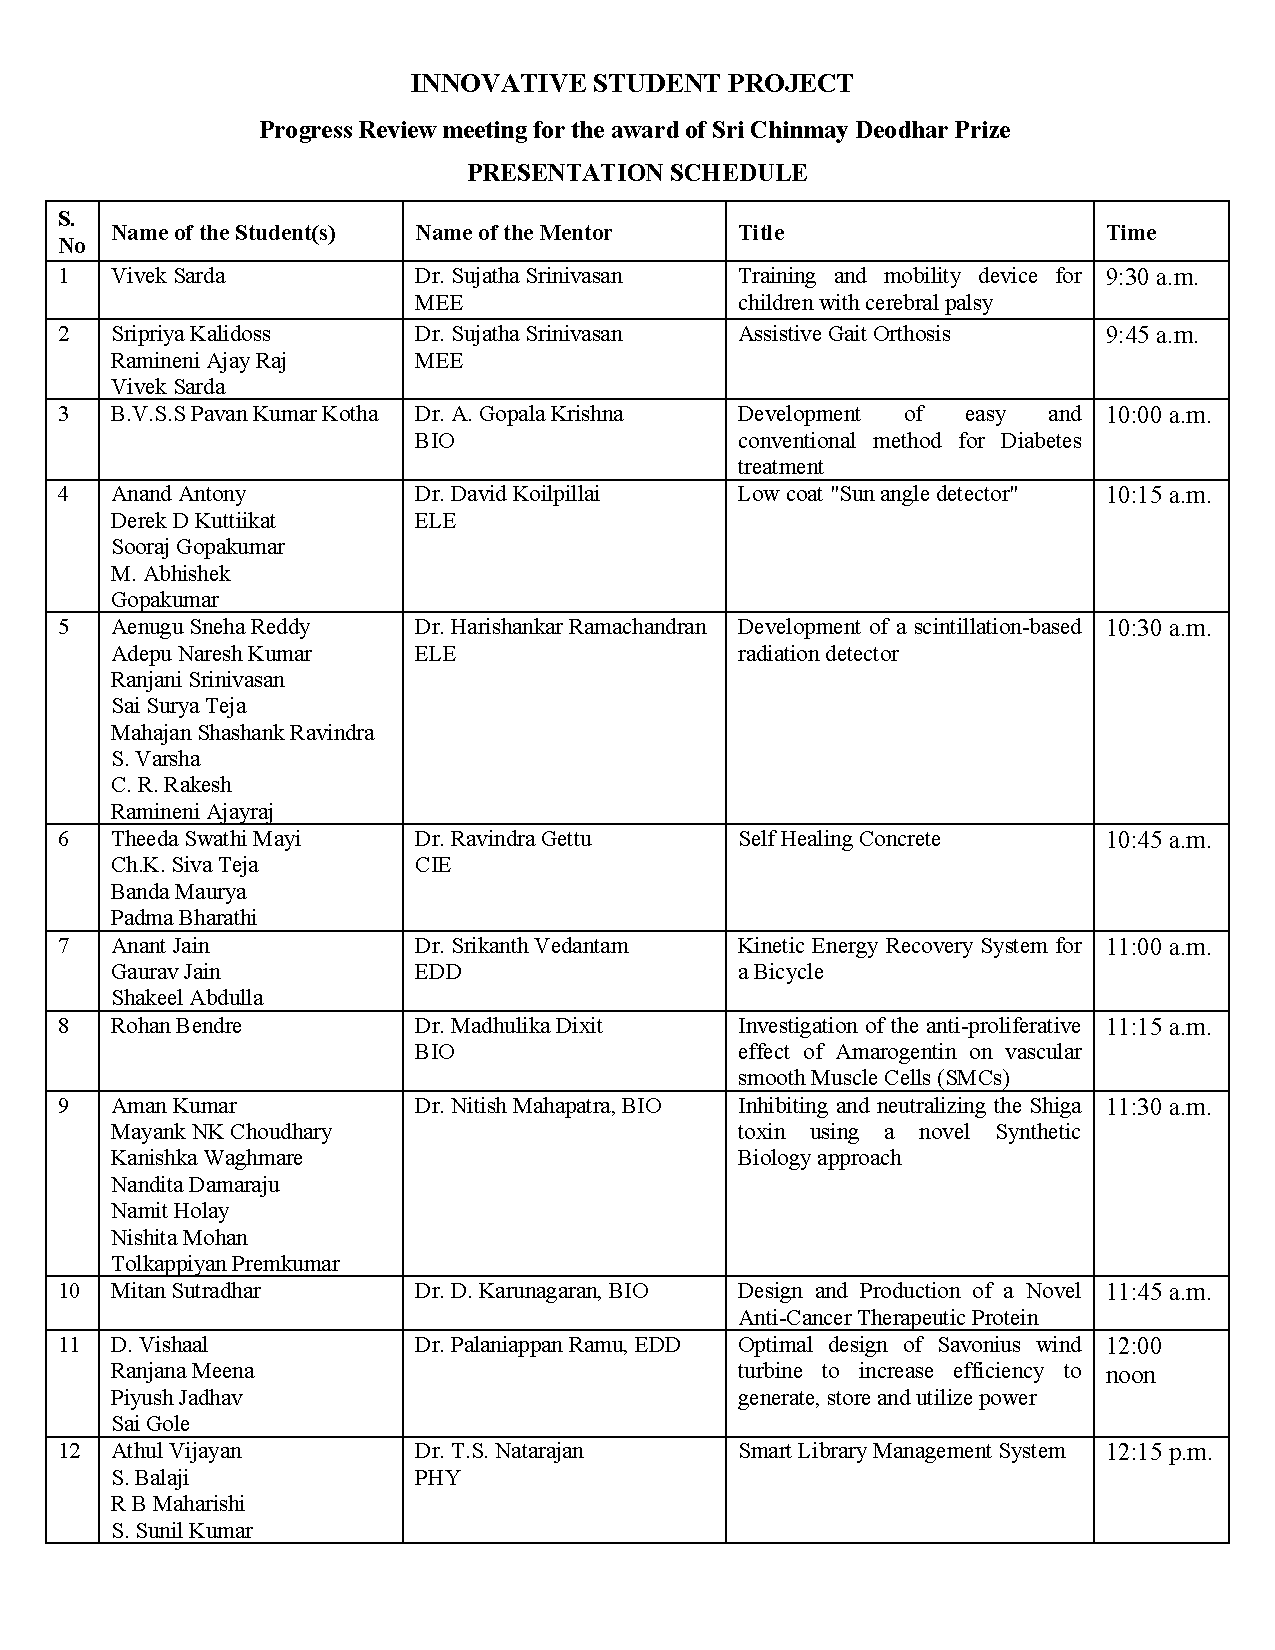
\includegraphics[width=\linewidth]{icsrreview.pdf}
    \caption{Review notice}
\end{subfigure}
\caption{ICSR project review notice}
\label{gauss}
\end{figure}
\FloatBarrier



\section{TI analog design contest}
\begin{figure}[h]
\centering

\includegraphics[width=0.8\textwidth]{adc.pdf}
\caption{TI analog design contest}
\label{gauss}
\end{figure}
\FloatBarrier

\section{TAS}
I guess you will have a list. this is a TAS contact details list from CFI. If more is required, let me know by PC.
\begin{figure}[h]
\centering
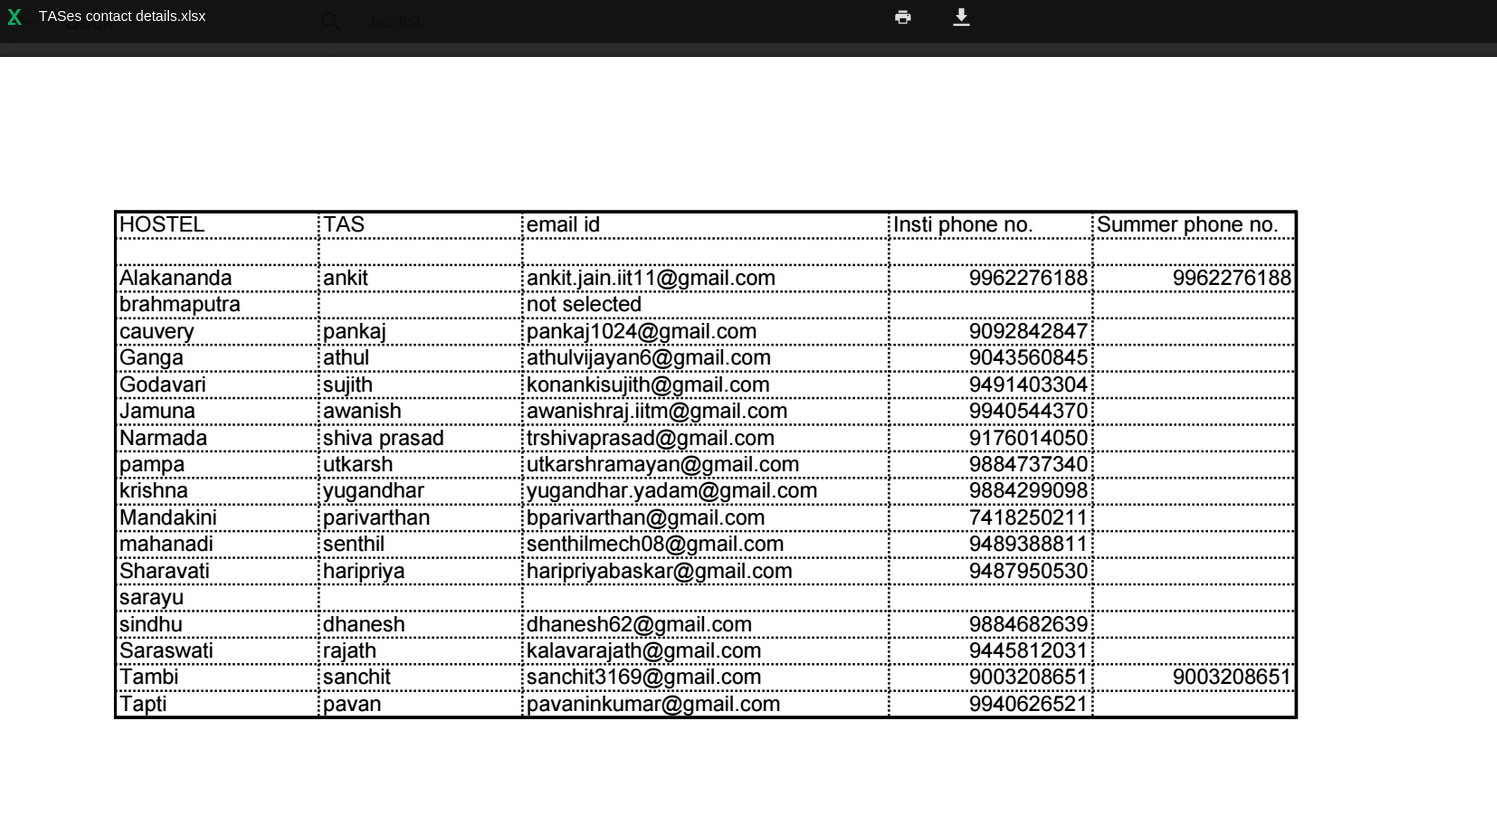
\includegraphics[width=0.8\textwidth]{taslist.png}
\caption{TAS certificate}
\label{gauss}
\end{figure}
\FloatBarrier 

\section{Shaastra coord and vol} % (fold)
\label{sec:shaastra_coord_and_vol}
Hope you have the list.

% section shaastra_coord_and_vol (end)   
\end{document}